\begin{center}
	\begin{tabular}{M{9.25cm}M{8.75cm}}
		\textbf{TRƯỜNG THCS-THPT NGUYỄN KHUYẾN}& \textbf{ÔN TẬP KTTX LẦN 1 - HỌC KÌ 2}\\
		\textbf{MÃ ĐỀ: 002}& \textbf{Bài thi môn: VẬT LÝ 10}\\
		\textit{(Đề thi có 04 trang)}& \textit{Thời gian làm bài: 40 phút, không kể phát đề}
		
		\noindent\rule{4cm}{0.8pt} \\
	\end{tabular}
\end{center}
\vspace{-0.5cm}
\setcounter{section}{0}
\section{Câu trắc nghiệm nhiều phương án lựa chọn}
\textit{Thí sinh trả lời từ câu 1 đến câu 12. Mỗi câu hỏi thí sinh chọn một phương án}
\setcounter{ex}{0}
\Opensolutionfile{ans}[ans/D10-KTTX3-002-TN]
% ===================================================================
\begin{ex}
	Câu nào sau đây là \textbf{không đúng}?
	\choice
	{\True Áp suất của chất lỏng không phụ thuộc vào khối lượng riêng của chất lỏng}
	{Độ tăng áp suất lên một bình kín truyền đi nguyên vẹn trong bình}
	{Độ chênh lệch áp suất tại hai vị trí khác nhau trong lòng chất lỏng không phụ thuộc áp suất khí quyển ở mặt thoáng}
	{Khi lặn xuống nước càng sâu thì ta chịu một áp suất càng lớn }
	\loigiai{}
\end{ex}
% ===================================================================
\begin{ex}
	\immini{Ba quả cầu bằng thép được nhúng vào trong nước như hình bên. Nhận xét nào sau đây là đúng về áp suất của nước lên các quả cầu?
		\choice
		{Áp suất lên quả 2 là lớn nhất vì có thể tích lớn nhất}
		{Áp suất lên quả 1 là lớn nhất vì có thể tích nhỏ nhất}
		{\True Áp suất lên quả 3 là lớn nhất vì sâu nhất}
		{Áp suất lên ba quả như nhau vì cùng bằng thép và cùng ở trong nước}}
	{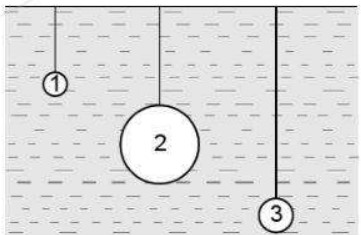
\includegraphics[scale=0.6]{../figs/D10-KTTX3-002-6}}
	\loigiai{}
\end{ex}
% ===================================================================
\begin{ex}
	\immini{Khi tác dụng một lực $\vec{F}$ vuông góc với cánh cửa, có độ lớn không đổi vào các vị trí khác nhau như hình bên. Moment lực gây ra tại vị trí nào là lớn nhất?	
		\choice
		{Điểm A}
		{Điểm B}
		{Điểm C}
		{\True Điểm D}}
	{\vspace{-0.75cm}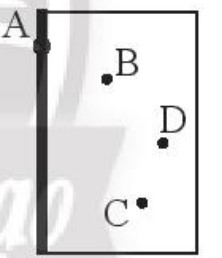
\includegraphics[scale=0.6]{../figs/D10-KTTX3-001-7}}
	\loigiai{}
\end{ex}
% ===================================================================
\begin{ex}
	Ở trường hợp nào sau đây, lực có tác dụng làm cho vật rắn quay quanh trục?
	\choice
	{Lực có giá nằm trong mặt phẳng vuông góc với trục quay và cắt trục quay}
	{Lực có giá song song với trục quay}
	{Lực có giá cắt trục quay}
	{\True Lực có giá nằm trong mặt phẳng vuông góc với trục quay và không cắt trục quay}
	\loigiai{}
\end{ex}
% ===================================================================
\begin{ex}
	Một vật rắn quay quanh trục thì tổng moment lực tác dụng lên vật có giá trị
	\choice
	{bằng không}
	{\True khác không}
	{luôn dương}
	{luôn âm}
	\loigiai{}
\end{ex}
% ===================================================================
\begin{ex}
	Chọn câu đúng.\\
	Cánh tay đòn của một lực $\vec{F}$ đến trục quay O là
	\choice
	{khoảng cách từ trục quay O đến ngọn của vector lực}
	{khoảng cách từ điểm đặt của lực đến trục quay}
	{\True khoảng cách từ trục quay O đến đường thẳng mang vector lực $\vec{F}$}
	{khoảng cách từ trục quay O đến một điểm trên vector lực}
	\loigiai{}
\end{ex}
% ===================================================================
\begin{ex}
	Moment của một lực $\vec{F}$ nằm trong mặt phẳng vuông góc với trục quay là
	\choice
	{đại lượng đặc trưng cho tác dụng làm quay quanh trục ấy}
	{đo bằng tích số giữa độ lớn của lực với cánh tay đòn}
	{đơn vị $\si{\newton\cdot\meter}$}
	{\True Cả ba đáp án trên}
	\loigiai{}
\end{ex}
% ===================================================================
\begin{ex}
	Cửa ngoài của một nhà rộng $\SI{3.4}{\meter}$ cao $\SI{2.1}{\meter}$. Một trận bão đi qua, áp suất bên ngoài giảm còn $\SI{0.96}{atm}$. Trong nhà áp suất vẫn giữa ở $\SI{1.0}{atm}$, áp lực toàn phần ép vào của là
	\choice
	{\SI{5.78E4}{\newton}}
	{\SI{1.45E4}{\newton}}
	{\True \SI{2.89E4}{\newton}}
	{\SI{4.34E4}{\newton}}
	\loigiai{}
\end{ex}
% ===================================================================
\begin{ex}
Khối lượng riêng của nước biển là \SI{1.0E3}{\kilogram/\meter^3}, áp suất khí quyển $p_0=\SI{1.01E5}{\newton/\meter^2}$ thì ở độ sâu \SI{1000}{\meter} dưới mực nước biển có áp suất tuyệt đối là	
	\choice
	{\SI{E8}{\pascal}}
	{\True \SI{E7}{\pascal}}
	{\SI{99.01E5}{\pascal}}
	{\SI{E9}{\pascal}}
	\loigiai{}
\end{ex}
% ===================================================================
\begin{ex}
	Một thanh chắn đường dài \SI{7.8}{\meter} có trọng lượng \SI{210}{\newton} và có trọng tâm cách đầu bên trái \SI{1.2}{\meter}. Thanh có thể quay quanh một trục nằm ngang ở cách đầu bên trái \SI{1.5}{\meter}. Để thanh nằm ngang thì cần tác dụng vào đầu bên phải một lực có độ lớn là
	\begin{center}
		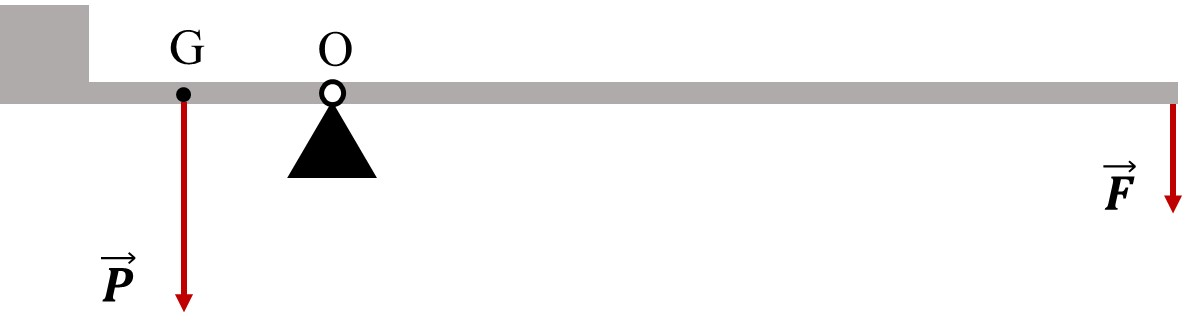
\includegraphics[scale=0.5]{../figs/D10-KTTX3-002-8}
	\end{center}
	\choice
	{\SI{20}{\newton}}
	{\True \SI{10}{\newton}}
	{\SI{30}{\newton}}
	{\SI{40}{\newton}}
	\loigiai{}
\end{ex}
% ===================================================================
\begin{ex}
	Một viên bi sắt có thể tích \SI{5E-7}{\meter^3} được thả rơi trong dầu. Lực cản do dầu tác dụng lên viên bi có độ lớn phụ thuộc vào tốc độ $v$ của bi dạng $F_c=0,1v$. Khối lượng riêng của sắt và dầu lần lượt là \SI{7890}{\kilogram/\meter^3} và \SI{890}{\kilogram/\meter^3}. Lấy gia tốc trọng trường $g=\SI{9.8}{\meter/\second^2}$. Tốc độ bão hòa của viên bi là
	\choice
	{\True \SI{0.34}{\meter/\second}}
	{\SI{0.39}{\meter/\second}}
	{\SI{0.04}{\meter/\second}}
	{\SI{0.43}{\meter/\second}}
	\loigiai{}
\end{ex}
% ===================================================================
\begin{ex}
Một cân đòn sử dụng khối lượng trượt \SI{100}{\gram} để cân vật M. Cân đạt được sự cân bằng khi hệ vật nằm ở vị trí như hình bên dưới. Khối lượng của vật M được cân trong trường hợp này là
\begin{center}
	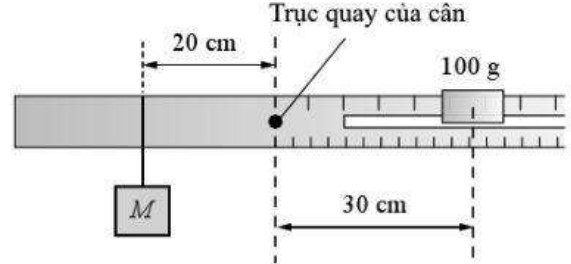
\includegraphics[scale=0.6]{../figs/D10-KTTX3-002-5}
\end{center}
		\choice
		{\True \SI{150}{\gram}}
		{\SI{66.7}{\gram}}
		{\SI{500}{\gram}}
		{\SI{100}{\gram}}
	\loigiai{}
\end{ex}
\Closesolutionfile{ans}
\section{Câu trắc nghiệm đúng/sai} 
\textit{Thí sinh trả lời từ câu 1 đến câu 4. Trong mỗi ý \textbf{a)}, \textbf{b)}, \textbf{c)}, \textbf{d)} ở mỗi câu, thí sinh chọn đúng hoặc sai}
\setcounter{ex}{0}\\
\Opensolutionfile{ans}[ans/D10-KTTX3-002-TF]
% ===================================================================
\begin{ex}
\immini{Trong các phát biểu sau, phát biểu nào đúng, phát biểu nào sai?	
	\choiceTF
	{\True Người ta làm các mũi kim nhọn để tăng áp suất giúp nó dễ xuyên qua vải}
	{Khi qua các đường lầy lội, người ta hay đặt các tấm ván giúp tăng áp suất để người và xe đi lại dễ dàng}
	{\True Bánh xe của các xe tăng được thiết kế dạng bánh xích to rộng để giảm áp suất của xe lên mặt đường}
	{\True Trong hai cái xẻng như hình bên thì xẻng đầu nhọn dễ xúc đất hơn}}
	{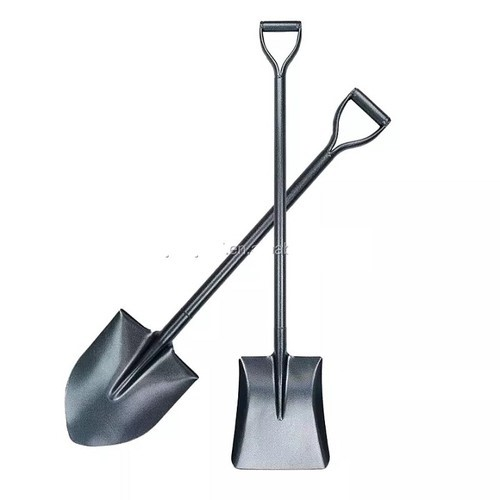
\includegraphics[scale=0.3]{../figs/D10-KTTX3-002-7}}
	\loigiai{}
\end{ex}
% ===================================================================
\begin{ex}
	\immini{Hình bên mô tả chuyển động của người nhảy dù ở 4 giai đoạn:
		\begin{enumerate}[label=Hình \alph*), leftmargin=2cm]
			\item Khi vừa mới nhảy.
			\item Chuyển động ổn định.
			\item Vừa bung dù.
			\item Chuyển động ổn định.
		\end{enumerate}
		\choiceTF
		{\True Trong quá trình rơi khi chưa bung dù, lực cản tác dụng lên người có độ lớn tăng dần cho đến khi người đạt tốc độ giới hạn}
		{Trong quá trình kể từ khi nhảy đến khi đạt tốc độ giới hạn, người nhảy dù rơi nhanh dần đều}
		{Sau khi bung dù, người nhảy dù chuyển động chậm dần đều do độ lớn lực cản lớn hơn trọng lực}
		{\True Ở giai đoạn chuyển động ổn định, lực cản tác dụng lên người và dù có độ lớn không đổi}
	}
	{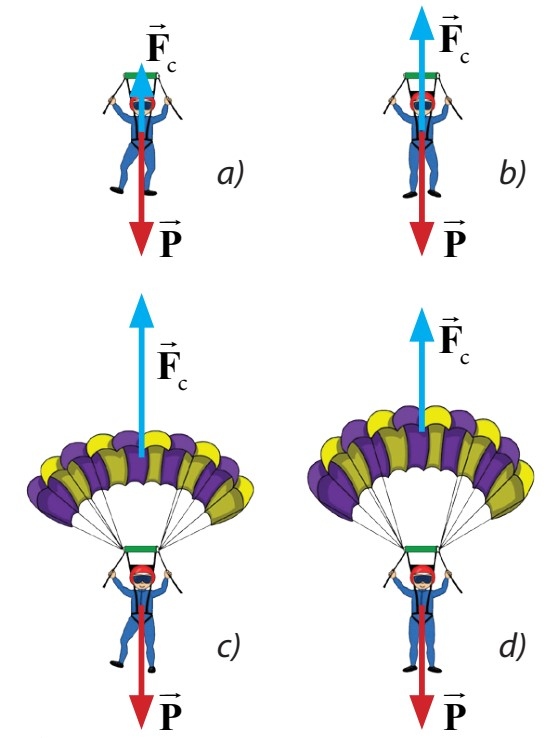
\includegraphics[scale=0.55]{../figs/D10-KTTX3-001-1}}
	\loigiai{}
\end{ex}
% ===================================================================
\begin{ex}
	\immini{Nhóm học sinh thực hiện thí nghiệm kiểm chứng quy tắc moment lực với các dụng cụ thí nghiệm như hình bên. Một đĩa tròn có trục quay đi qua tâm O, trên mặt đĩa có những lỗ ghim để treo các quả cân. Dây CD được vắt qua ròng rọc cố định R.\choiceTF
		{\True Trọng lực của đĩa không có tác dụng làm cho đĩa quay}
		{\True Nếu treo tại B và D mỗi bên 1 quả cân như hình, thì đĩa có xu hướng quay ngược chiều kim đồng hồ}
		{Nếu treo 1 quả cân tại B thì cần treo 3 quả cân tại D để đĩa không quay}
		{Khi đĩa cân bằng, hợp lực của lực căng 2 dây bằng trọng lượng của đĩa}}
	{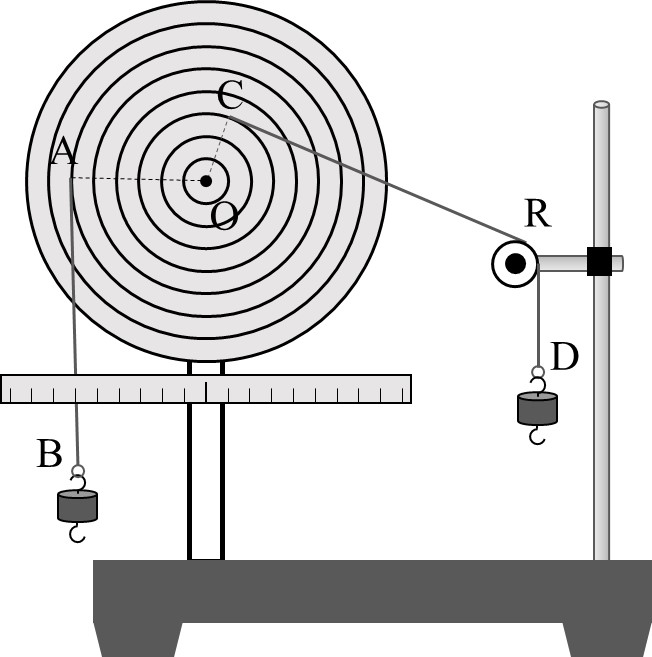
\includegraphics[scale=0.5]{../figs/D10-KTTX3-002-3}}
	
	\loigiai{}
\end{ex}
% ===================================================================
\begin{ex}
	Để vận chuyển cống bê tông cốt thép hình trụ có trọng lượng \SI{24}{\kilo\newton} đến công trình xây dựng một cách an toàn, người ta đặt cống lên 2 nêm I và II như hình vẽ bên. Xét trong quá trình xe đang chuyển động thẳng đều, cống và các nêm nằm yên trên sàn xe.	
	\immini{\choiceTF
		{\True Phản lực do các mặt nêm tác dụng lên cống có phương qua tâm cống}
		{\True Phản lực do mặt nêm (I) tác dụng lên cống có độ lớn $\xsi{12\sqrt{3}}{\kilo\newton}$}
		{Đối với trục quay qua điểm tiếp xúc giữa cống và nêm (I), moment của phản lực do mặt nêm (II) tác dụng lên cống bằng không}
		{\True Phản lực do mặt nêm (II) tác dụng lên cống có độ lớn $\SI{12}{\kilo\newton}$}}
	{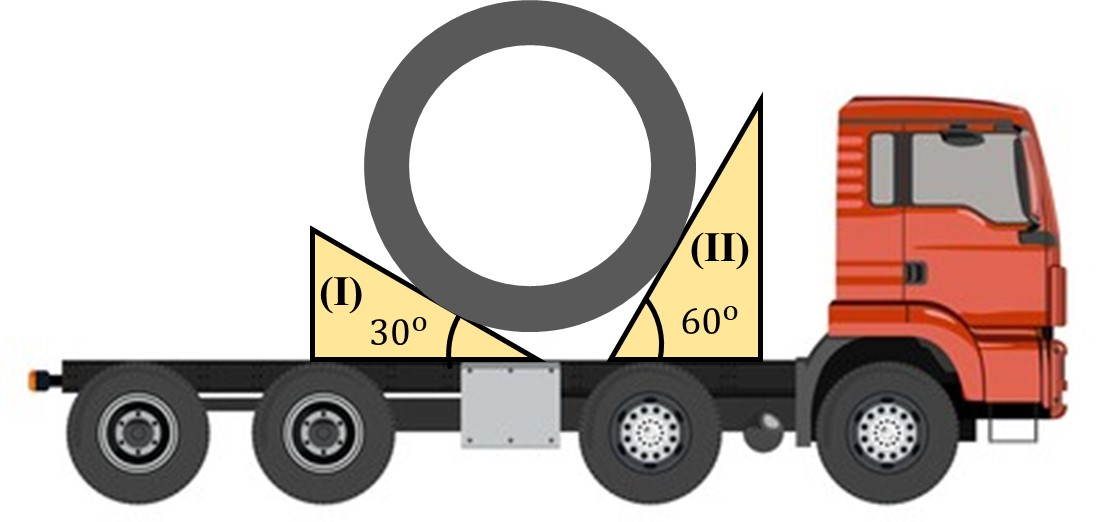
\includegraphics[scale=0.4]{../figs/D10-KTTX3-002-4}}
	\loigiai{}
\end{ex}
\Closesolutionfile{ans}
\section{Tự luận}
\setcounter{ex}{0}
\Opensolutionfile{ans}[ans/D10-KTTX3-002-TL]
% ======================================================================
\begin{ex} \textit{(2,0 điểm)}
\immini{	Tiến trang trí nhà cửa để chuẩn bị đón Tết Nguyên Đán 2025. Phía trước nhà, Tiến cần treo cặp đèn lồng, mỗi chiếc đèn có khối lượng $\SI{1.8}{\kilogram}$. Đèn lồng được treo ở đầu thanh kim loại đồng chất, tiết diện đều, có thể quay quanh bản lề tại O như hình vẽ. Để thanh cân bằng, đầu A của thanh cần được gắn với tường bằng sợi dây AB nhẹ, không dãn, dây làm với tường góc $\SI{60}{\degree}$. Lấy gia tốc trọng trường $g=\SI{10}{\meter/\second^2}$. Em hãy xác định độ lớn của lực căng trên dây AB trong các trường hợp sau:
	\begin{enumerate}[label=\alph*)]
		\item thanh OA nhẹ.
		\item thanh OA có khối lượng $\SI{1.2}{\kilogram}$.
\end{enumerate}}
{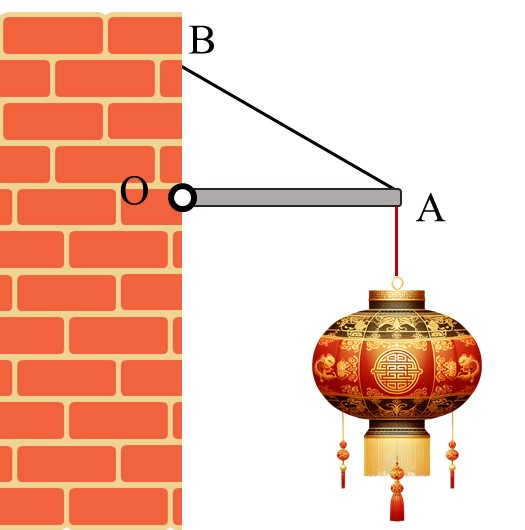
\includegraphics[scale=0.5]{../figs/D10-KTTX3-002-1}}
		\loigiai{}
\end{ex}
% ======================================================================
\begin{ex} \textit{(1,0 điểm)}
\immini{	Dịch não tủy là chất lỏng tồn tại trong các não thất và tủy sống, có vai trò quan trọng trong việc bảo vệ não, lấy các nguồn dinh dưỡng cần thiết từ máu cung cấp cho não và loại bỏ các chất thải từ các tế bào não. Dịch não tủy lưu chuyển giữa các khoang sọ và cột sống, tạo ra áp suất cao hơn áp suất khí quyển từ \SI{100}{\milli\meter\ce{H_2O}} đến \SI{200}{\milli\meter\ce{H_2O}}. Trong y tế, áp suất thường được đo bằng đơn vị \si{\milli\meter\ce{H_2O}} vì dịch cơ thể (bao gồm cả dịch não tủy) có khối lượng riêng gần bằng khối lượng riêng của nước. }
{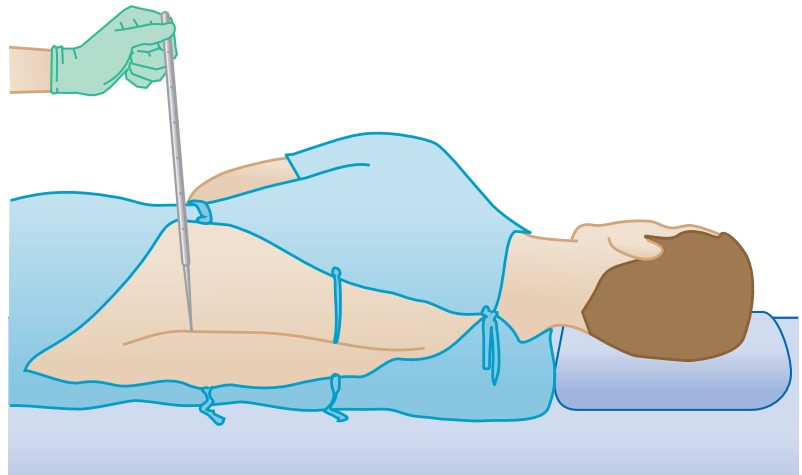
\includegraphics[scale=0.4]{../figs/D10-KTTX3-002-2}}
Áp suất của dịch não tủy có thể được xác định bằng phương pháp "chọc dò tủy sống". Một ống rỗng được đưa vào cột sống của bệnh nhân và chiều cao mà chất lỏng dâng lên được quan sát như hình bên. Lấy khối lượng riêng của nước $\rho=\SI{1000}{\kilogram/\meter^3}$, gia tốc trọng trường $g=\SI{9.8}{\meter/\second^2}$.
	\begin{enumerate}[label=\alph*)]
		\item Nếu chiều cao cột chất lỏng dâng lên trong ống là $\SI{160}{\milli\meter}$ thì áp suất của dịch não tủy cao hơn áp suất khí quyển bao nhiêu pascal?
		\item Trong một số trường hợp, chẳng hạn bệnh nhân bị chấn thương dẫn đến dập đốt sống làm tắc nghẽn dòng chảy của dịch não tủy hoặc bác sĩ nghi ngờ về sự phát triển của khối u xâm lấn cột sống và ức chế dòng chảy của dịch não tủy, bác sĩ có thể làm nghiệm pháp Queckensted. Trong thủ thuật này, người ta ấn hai bên tĩnh mạch cổ của bệnh nhân trong thời gian 30 giây khiến huyết áp trong não tăng lên. Nếu bệnh nhân bình thường, điều gì sẽ xảy ra với mực chất lỏng trong ống chọc tủy sống? Giải thích.
	\end{enumerate} 
	\loigiai{}
\end{ex}
\Closesolutionfile{ans}
\begin{center}
	\textbf{--- HẾT ---}
\end{center}